\documentclass[tikz,border=5mm]{standalone}
\usepackage[utf8]{vietnam}
\usepackage{tikz,tkz-euclide,tkz-tab,enumerate}
\usetikzlibrary{shapes,calc,intersections,angles,patterns,quotes}
\usetkzobj{all}
\begin{document}
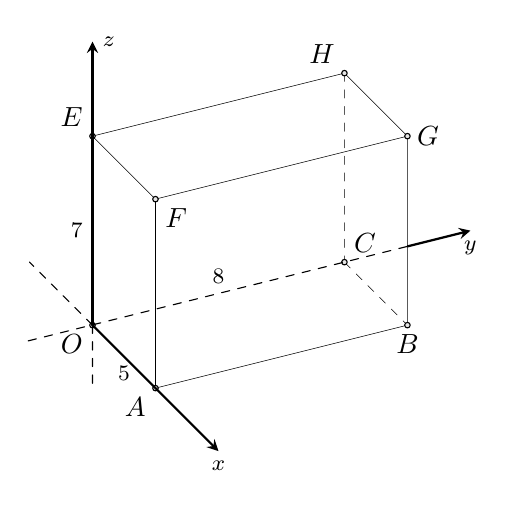
\begin{tikzpicture}[scale=0.8, line join=round, line cap=round,>=stealth]

			\tkzDefPoints{0/0/O, 1/-1/A, 4/1/C}

			\coordinate (B) at ($(A)+(C)-(O)$);

			\coordinate (E) at ($(O)+(0,3)$);

			\coordinate (F) at ($(E)+(A)-(O)$);

			\coordinate (G) at ($(E)+(B)-(O)$);

			\coordinate (H) at ($(E)+(C)-(O)$);

			\tkzDrawSegments(O,A A,B B,G G,F F,A G,H H,E E,F)

			\tkzDrawSegments[dashed](H,C C,B)

			\tkzDrawPoints(O,A,B,C,E,F,G,H)

			\tkzLabelSegment[below](O,A){\footnotesize $5$}

			\tkzLabelSegment[above](O,C){\footnotesize $8$}

			\tkzLabelSegment[left](O,E){\footnotesize $7$}

			\tkzLabelPoints[below left](O,A)

			\tkzLabelPoints[below](B)\tkzLabelPoints[above left](E,H)\tkzLabelPoints[above right](C)\tkzLabelPoints[right](G)\tkzLabelPoints[below right](F)

			\draw[dashed](-1.02,-0.25)--(5,1.25);

			\draw[dashed] (0,0)--(0,-1) (0,0)--(-1,1);

			\draw[->,thick] (0,0)--(2,-2) node [below] {\footnotesize $x$};

			\draw[->,thick] (0,0)--(0,4.5)node [right] {\footnotesize $z$};

			\draw[->,thick] (5,1.25)--(6,1.5)node [below] {\footnotesize $y$};

	\end{tikzpicture}
\end{document}